% Result evaluation
\chapter{Submodule benchmarks}

While the last chapter discussed the implementation details of the different modules, this chapter will present the results of the performance measurements. One of the key concerns for a game engine is performance and that is the reason why it is the computation time of several benchmark scenarios that is compared. The results and findings of the measurement process are then visualized to show where the performance of the implementations diverge and where they are on the same level. Starting with a description of the benchmark process and the environment, the first part will also list the scenarios that were measured. 

\section{Benchmark setup}

\subsection{Time measurement}

Retrieving fine-grained and reliable timestamps is important when comparing different implementations against each other. To measure elapsed time the first naive solution would be to use a facility such as the \texttt{time()} function from the C standard library. But since \texttt{time()} only returns the elapsed seconds since the first January 1970 \cite{C_Time}, a more precise method is required. A possible solution can be a high-resolution timer on a CPU. Because this kind of timer uses a register to store the amount of cycles passed since the CPU was started, it is possible to generate more precise timestamps yielding better resolution of differences between them. The option chosen for measuring time on the Windows \ac{OS} is \texttt{QueryPerformanceCounter()} from the \textit{Win32 \ac{API}}.

\subsection{Environments}

The benchmark process is run on two different hardware setups. The following tables describe the hardware on these machines and group them under a name per environment. The following sections will use these names to refer to the different environments.

\begin{table}[h!]
	\centering
	\label{my-label}
	\begin{tabular}{|l|l|l|}
		\hline
		\textbf{Environment name} & \textbf{Processor / CPU} & \textbf{RAM} \\ \hline
		Mobile Workstation	& \textit{Processor	Intel(R) Core(TM) i7-6700 @ 3.40GHz, 4 Cores} & \textit{16 GB} \\ \hline
		Razer Blade Stealth	& \textit{Processor	Intel(R) Core(TM) i7-7500U @ 2.70 GHz, 2 Cores} & \textit{16 GB} \\ \hline
	\end{tabular}
	\caption{Benchmark environment names and hardware capabilities}
\end{table}

\subsection{Benchmark applications}

To measure the different scenarios that are listed in the next section, every project includes an application that is able to run them. In order to yield minimal overhead when choosing benchmark scenarios, every executable includes a static lookup table where the function pointers to the scenarios are stored. Each scenario has an id which also serves as an index into the lookup table. When the application is started the id is passed as a command-line parameter. This behavior was chosen to allow the author to automate the benchmark process via command-line scripts. Listing \ref{lst:cpp_bench_app} shows how the C++ main function of a benchmark application looks like. At the end it can be seen, that the scenario id passed as a command-line argument is converted into an integer and then used to index into the scenario table. The signature of every benchmark scenario has to follow the one defined as \texttt{typedef void(*BenchmarkScenarioFunction)()}. The Rust benchmark main function works similar to the C++ one.\\

\begin{lstlisting}[caption={Main function of the C++ benchmark app using a scenario lookup table}, label={lst:cpp_bench_app}, language={C++}]
int main(int argc, char** argv)
{
	if (argc <= 1 || argc > 2)
	{
		std::cerr << "Usage: bench_spark++.exe SCENARIO_ID" << std::endl;
		return -1;
	}
	
	scenarios[atoi(argv[1])]();
}
\end{lstlisting}

\noindent

Additional to the two benchmark applications the author implemented a test automation and measurement tool in Rust. \textit{SparkX} is a command-line application able to run other executables and measure them. Beside that, it is also possible to collect the output of the started processes. In the context of the thesis the tool was used to run a benchmark scenario thousand times and later average the results of the specific benchmark application. \textit{SparkX} is also capable of formatting the results in a comma-separated form, making it easy to import the created results into tools such as Microsoft Excel. Each result set contains the average scenario time, the lower and the upper bound of the measurements. \textit{SparkX} was a helpful utility to automate the benchmark process even more, making it easier for the author to run every scenario thousand times, creating more reasonable numbers.

\subsection{Scenarios}

To measure the performance of the different systems the following benchmark scenarios were implemented. 

\subsubsection{Memory management}

\begin{enumerate}
	\item \textbf{RawAllocators}: one scenario was implemented per allocator to test raw allocations with the natural alignment of a common struct. Every scenario allocates 1000 elements. Beside the custom allocators the measurement includes the default dynamic heap allocation systems from the two languages.
	
	\item \textbf{MemoryRealm\_LinearAllocator}: a scenario where 1000 small object allocations are made via a memory realm. The realm includes a linear allocator and uses simple bounds checking.
\end{enumerate}

\subsubsection{Container}

\begin{enumerate}
	\item \textbf{VecDefault}: push 10000 small objects into a vector with no previous capacity, forcing it to grow
	
	\item \textbf{VecCapacity}: push 10000 small objects into a vector with previously requested capacity
	
	\item \textbf{VecIteration}: push 10000 small objects into a vector with previously requested capacity and iterate them afterwards 

	\item \textbf{VecErase}: push 10000 small objects into a vector with previously requested capacity and erase them one by one afterwards
	
	\item \textbf{HandleMapInsertion}: insert 10000 small objects into the handle map
	
	\item \textbf{HandleMapIteration}: insert 10000 small objects into the handle map and iterate them afterwards
	
	\item \textbf{HandleMapRemove}: insert 10000 small objects into the handle map and remove them afterwards one by one
	
	\item \textbf{RingbufferWrite}: insert 10000 small objects into the ringbuffer until it is full

	\item \textbf{RingbufferRead}: insert 10000 small objects into the ringbuffer and consume them all
	
	\item \textbf{RingbufferWrite\_Wrapping}: insert 15000 objects into the ringbuffer overwriting the oldest 5000	
\end{enumerate}

\subsubsection{Entity Component System}

\begin{enumerate}
	\item \textbf{Position}: create 10000 entities and add a position component to each of them
	
	\item \textbf{PositionVelocity}: create 10000 entities with one position and one velocity component
	
	\item \textbf{Iteration}: iterate over 10000 position components of previously created entities
	
	\item \textbf{Remove}: create 10000 entities with position components and remove 5000 components afterwards
\end{enumerate}

\clearpage

\section{Results}

\subsection{Memory Management}

Considering the benchmarks shown in Figure \ref{fig:mem_bench_workstation} and Figure \ref{fig:mem_bench_blade}, the C++ version of the memory system performs better than the Rust implementation. Execution times of the Rust allocators are slightly slower than the C++ ones, but they only differ in a range from five to 50 microseconds. The pool allocator on the mobile workstation and the linear memory realm on the razor blade stealth performed better than C++ variants but only by a few microseconds. While the code of both implementations is rather similar, the Rust implementation contains more explicit type conversions and uses the \texttt{transmute} function to reinterpret types as others. The C++ implementation uses the \texttt{pseudo\_cast} utility, a wrapper around an \texttt{union} holding the template types. 

A baseline for the general performance of the allocator system is the first data-set in the graph that shows the execution time of the default allocators of the two languages. In C++ that facility was \texttt{new} while the Rust variant uses \texttt{Box} to dynamically allocate memory. It can be seen that the custom allocators generally perform better than the respective default ones. This comparison is not significant for the difference between Rust and C++, but supports the theory that custom allocators can enhance the performance of a game engine.

\begin{figure}[h!]
	\centering
	\begin{subfigure}[b]{\textwidth}
		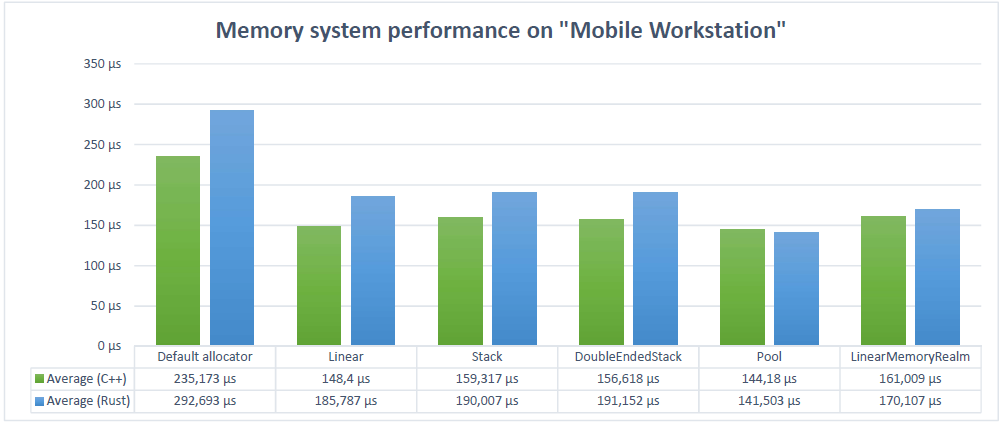
\includegraphics[width=1\linewidth]{PICs/mem_bench_workstation.png}
		\caption{Visual comparison of the different allocators, in Rust and C++}
		\label{fig:mem_bench_workstation} 
	\end{subfigure}
	
	\begin{subfigure}[b]{\textwidth}
		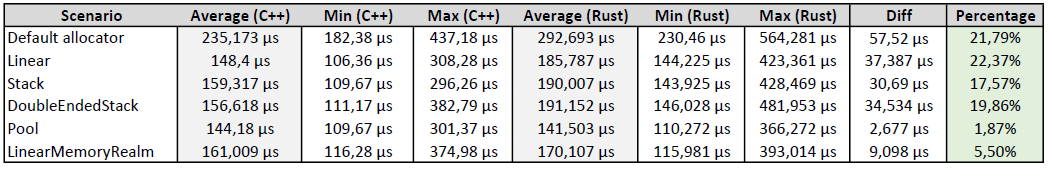
\includegraphics[width=1\linewidth]{PICs/mem_bench_workstation_data.png}
		\caption{Exact measurements of the benchmarks, in microseconds}
		\label{fig:mem_bench_blade}
	\end{subfigure}
	
	\caption[Memory benchmarks workstation]{Memory system benchmarks on the mobile workstation configuration}
\end{figure}

\clearpage

\begin{figure}[h!]
	\centering
	\begin{subfigure}[b]{\textwidth}
		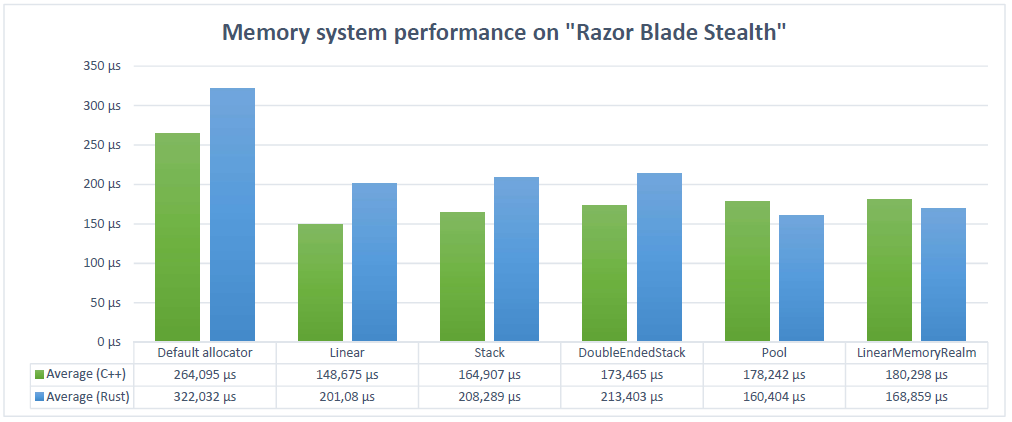
\includegraphics[width=1\linewidth]{PICs/mem_bench_blade.png}
		\caption{Visual comparison of the different allocators, in Rust and C++}
		\label{fig:Ng1} 
	\end{subfigure}
	
	\begin{subfigure}[b]{\textwidth}
		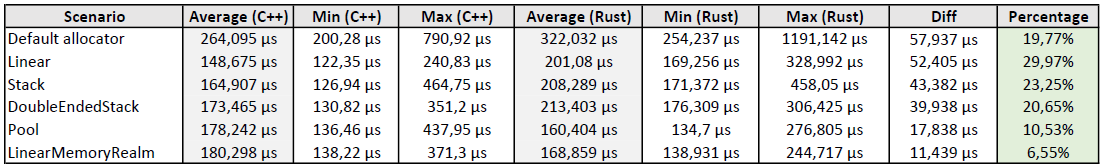
\includegraphics[width=1\linewidth]{PICs/mem_bench_blade_data.png}
		\caption{Exact measurements of the benchmarks, in microseconds}
		\label{fig:Ng2}
	\end{subfigure}
	
	\caption[Memory benchmarks blade]{Memory system benchmarks on the razor blade stealth configuration}
\end{figure}

\clearpage

\subsection{Container}

Based on the figures \ref{fig:cont_bench_work} \& \ref{fig:cont_bench_blade} the C++ version of the container library performs better than the Rust variant. The Rust vector is about 25\% to 30\% slower than the C++ version, mostly due to the way how the Rust vector writes the data into the internal array. It is first moved into the \texttt{push} method and then immediately written into a memory slot of the internal array while the C++ variant uses \texttt{placement new} to create a new instance of the object into vector's place. 
The handlemap implementation yields better results in C++, with an average difference of about 35\% to 40\% percent. One difference that introduces a small overhead in the Rust handlemap is the way dynamic memory for the internal arrays is allocated. Because the implementation's goal was to use stable features where possible, the allocation library for raw memory could not be used. To follow the way that would be used in idiomatic Rust, the author chose to use a vector to allocate the needed memory at runtime. 
The last container, the ringbuffer, performs slightly better in Rust, but only by a difference of four to seven microseconds. Because the internal behavior of the ringbuffer is rather trivial, no great performance differences were expected. Therefore the measurement results for this container proofed the expectations. 

\begin{figure}[h!]
	\centering
	\begin{subfigure}[b]{\textwidth}
		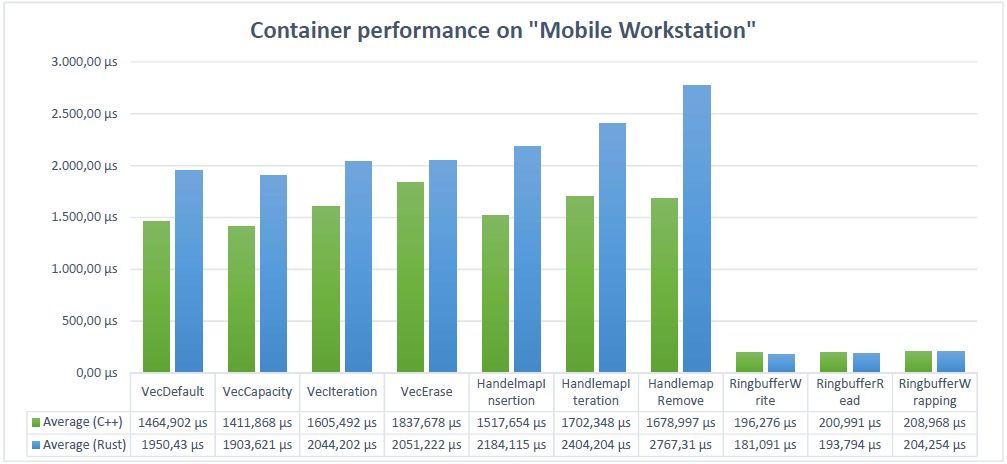
\includegraphics[width=1\linewidth]{PICs/container_bench_workstation.png}
		\caption{Visual comparison of the different containers, in Rust and C++}
		\label{fig:cont_bench_work} 
	\end{subfigure}
	
	\begin{subfigure}[b]{\textwidth}
		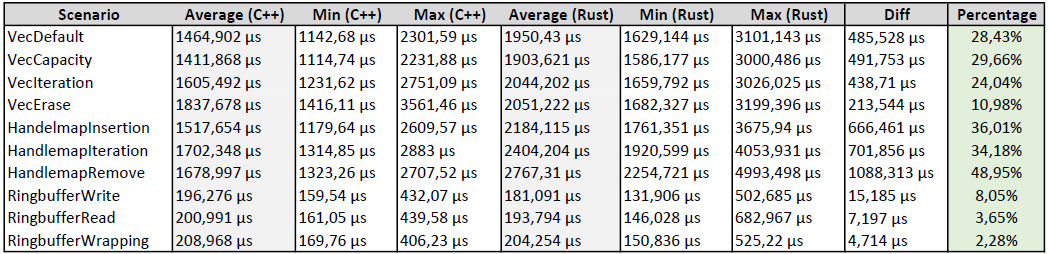
\includegraphics[width=1\linewidth]{PICs/container_bench_workstation_data.png}
		\caption{Exact measurements of the benchmarks, in microseconds}
		\label{fig:cont_bench_blade}
	\end{subfigure}
	
	\caption[Container benchmarks workstation]{Container benchmarks on the mobile workstation configuration}
\end{figure}

\clearpage

\begin{figure}[h!]
	\centering
	\begin{subfigure}[b]{\textwidth}
		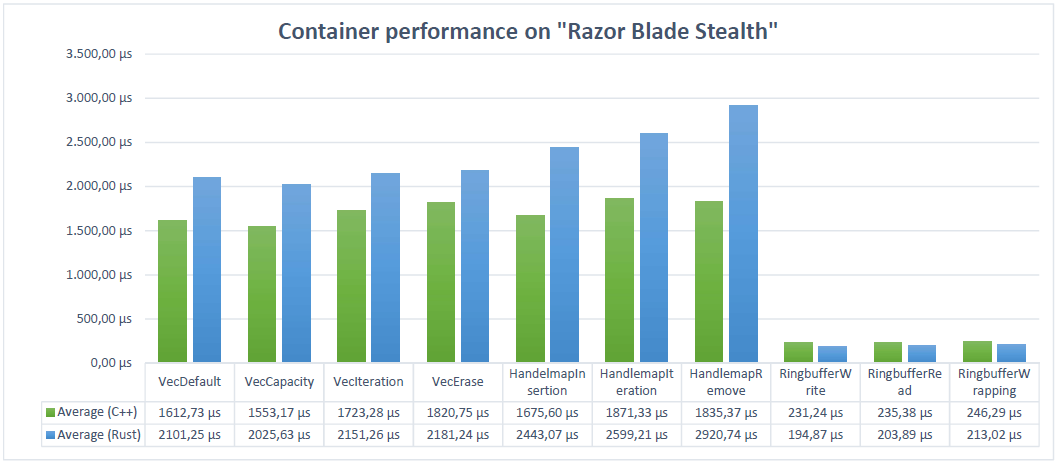
\includegraphics[width=1\linewidth]{PICs/container_bench_blade.png}
		\caption{Visual comparison of the different containers, in Rust and C++}
		\label{fig:Ng1} 
	\end{subfigure}
	
	\begin{subfigure}[b]{\textwidth}
		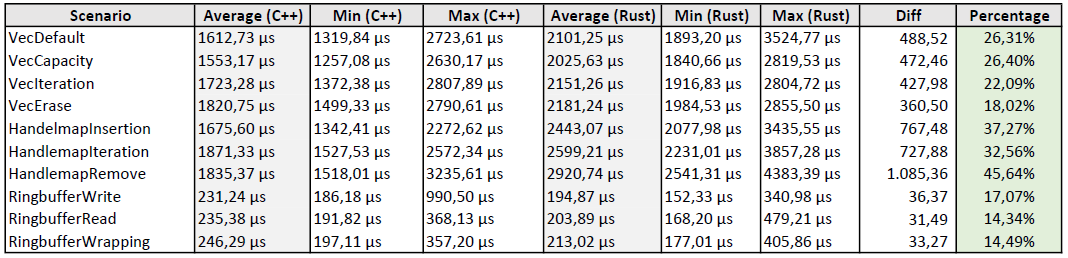
\includegraphics[width=1\linewidth]{PICs/container_bench_blade_data.png}
		\caption{Exact measurements of the benchmarks, in microseconds}
		\label{fig:Ng2}
	\end{subfigure}
	
	\caption[Container benchmarks blade]{Container benchmarks on the razor blade stealth configuration}
\end{figure}

\clearpage

\subsection{Entity Component System}

The results of the \ac{ECS} benchmark showed that the Rust implementation performs better than the C++ one. That difference is mostly due to the way the component storages were implemented in the Rust \ac{ECS} and how they work in the C++ variant. While in calx-ecs the creator provides a macro to register components with the \texttt{Ecs} type. It adds a field to the \texttt{Ecs} struct for every type a user registers. Because the macro system of Rust differs from the preprocessor-based one in C++, the reimplementation used a different approach. With C++ macros, the flexibility and amount of types that can be passed is constrained by macro expansion rules. When using variadic macros they need a distinct additional macro definition for every argument count. Because the Rust macro allows for theoretically unlimited registered component types, the C++ \ac{ECS} uses a hashmap that associates component storages with an unique component id. The lookup into that storage map introduces an overhead that could be avoided in Rust. Figures \ref{fig:ecs_bench_work} and \ref{fig:ecs_bench_blade} show these results and the second scenario benchmark also visualizes how in C++ the performance impact scales directly with the amount of components added to an entity, while the Rust performance does not scale in the same magnitude. 

\begin{figure}[h!]
	\centering
	\begin{subfigure}[b]{\textwidth}
		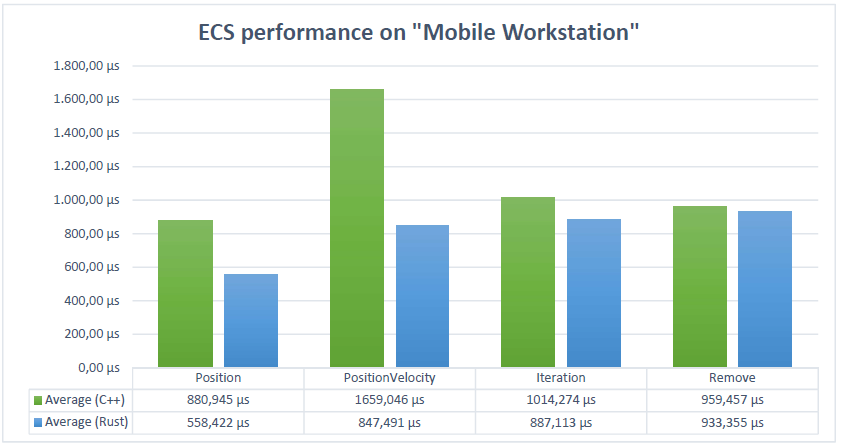
\includegraphics[width=1\linewidth]{PICs/ecs_bench_workstation.png}
		\caption{Visual comparison of the \ac{ECS} implementations, in Rust and C++}
		\label{fig:ecs_bench_work} 
	\end{subfigure}
	
	\begin{subfigure}[b]{\textwidth}
		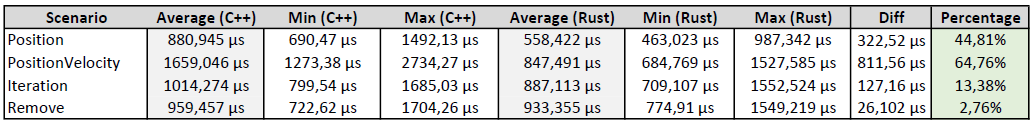
\includegraphics[width=1\linewidth]{PICs/ecs_bench_workstation_data.png}
		\caption{Exact measurements of the benchmarks, in microseconds}
		\label{fig:ecs_bench_work_data}
	\end{subfigure}
	
	\caption[ECS benchmarks workstation]{\ac{ECS} benchmarks on the mobile workstation configuration}
\end{figure}

\clearpage

\begin{figure}[h!]
	\centering
	\begin{subfigure}[b]{\textwidth}
		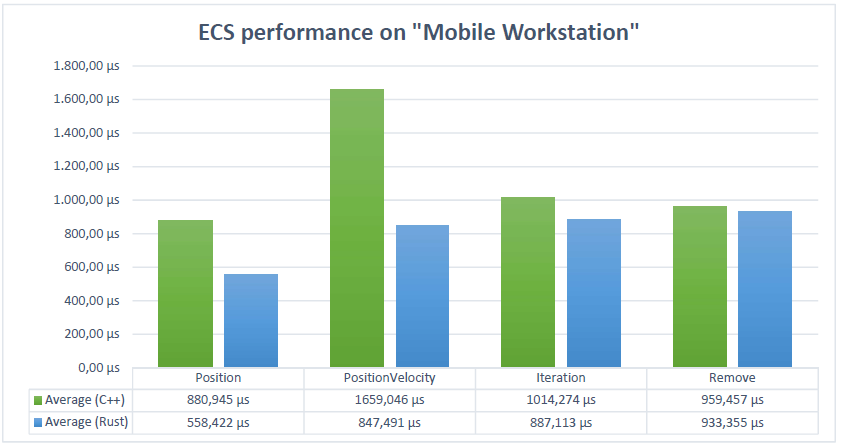
\includegraphics[width=1\linewidth]{PICs/ecs_bench_workstation.png}
		\caption{Visual comparison of the \ac{ECS} implementations, in Rust and C++}
		\label{fig:ecs_bench_blade} 
	\end{subfigure}
	
	\begin{subfigure}[b]{\textwidth}
		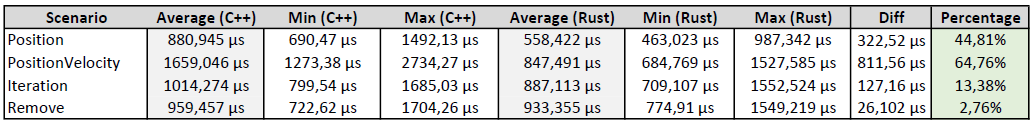
\includegraphics[width=1\linewidth]{PICs/ecs_bench_workstation_data.png}
		\caption{Exact measurements of the benchmarks, in microseconds}
		\label{fig:ecs_bench_blade_data}
	\end{subfigure}
	
	\caption[ECS benchmarks blade]{\ac{ECS} benchmarks on the razor blade stealth configuration}
\end{figure}